\chapter{Method}
At its core, our method formulates the necessary and sufficient conditions for quadrangulating a triangle-mesh by parametrization (integer-grid maps \cite{bommes:hal-00862648}), as a smooth unconstrained optimization problem using periodic functions. Our main objective function is a weighted sum of smooth sub-objective functions, of which their weights are controllable by the user. We believe that this approach is more suitable for 3D design and modeling tools since the quadrangulation process is continuous with the user constantly in the loop. This approach is also easily extensible by introducing additional sub-objectives smooth terms into the main objective, which can represent custom requirements of which the parameterization has to fulfill. Moreover, since the weights are controllable, the quadrangulation process can be executed in any desired order (e.g. achieve a seamless parametrization before handling singular points). That's why we decided  to call our approach \emph{Smooth and Interactive Parametrization-Based Quadrangulation}: \emph{Smooth} because we're using a smooth objective, \emph{Interactive} because small changes are immediately reflected to the user, and \emph{Parametrization-Based} because we solve a global parametrization problem. This chapter is organized as following: In section \ref{integer-grid-maps} we describe in detail the notion of inter-grid maps. In section \ref{label:quad_distortion_cond} we briefly describe how to we cope with quad-distortion in order to maximize mesh quality.
\section{Integer Grid Maps}
\label{integer-grid-maps}
The necessary and sufficient conditions for a parametrization mapping to form a valid quad mesh on the mesh's 3D surface are:
\begin{enumerate}
\item Seamless Condition
\item Singular Points Condition
\item Consistent Orientation Condition
\end{enumerate}
\subsection{Seamless Condition}
\label{label:seamless_cond}
The transition function $g_{ij}$ between two half-edges $e_i$ and $e_j$ on the parameterization domain that corresponds to the same surface edge that is part of a cut seam, has to be an integer-grid automorphism given by:
\begin{equation}\label{transition_g_ij}
\begin{split}
e_j = R^{r_{ij}}_{90^\circ}e_i + \vec{t}_{ij}
\end{split}
\end{equation}
Where  $r_{ij} \in \{0,1,2,3\}$ and $\vec{t}_{ij} \in \mathbb{Z}^2$. Figures \ref{fig:translation_req}, \ref{fig:angle_req} and \ref{fig:length_req} visually demonstrate the 3 requirements encoded by the seamless condition.
\begin{figure}[ht]
\centering
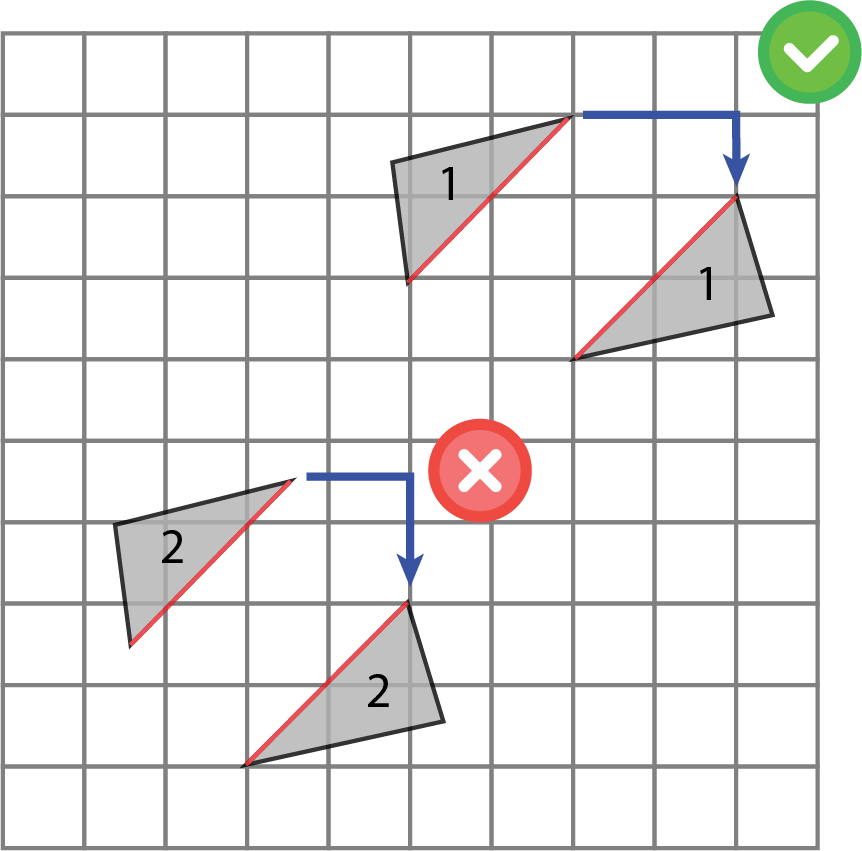
\includegraphics[width=9cm]{figures/seamless/translation.png}
\caption[The Translation Requirement]{The transition function $g_{ij}$, described by equation \ref{transition_g_ij}, should impose an integer translation between the two half edges.}
\label{fig:translation_req}
\end{figure}
\begin{figure}[ht]
\centering
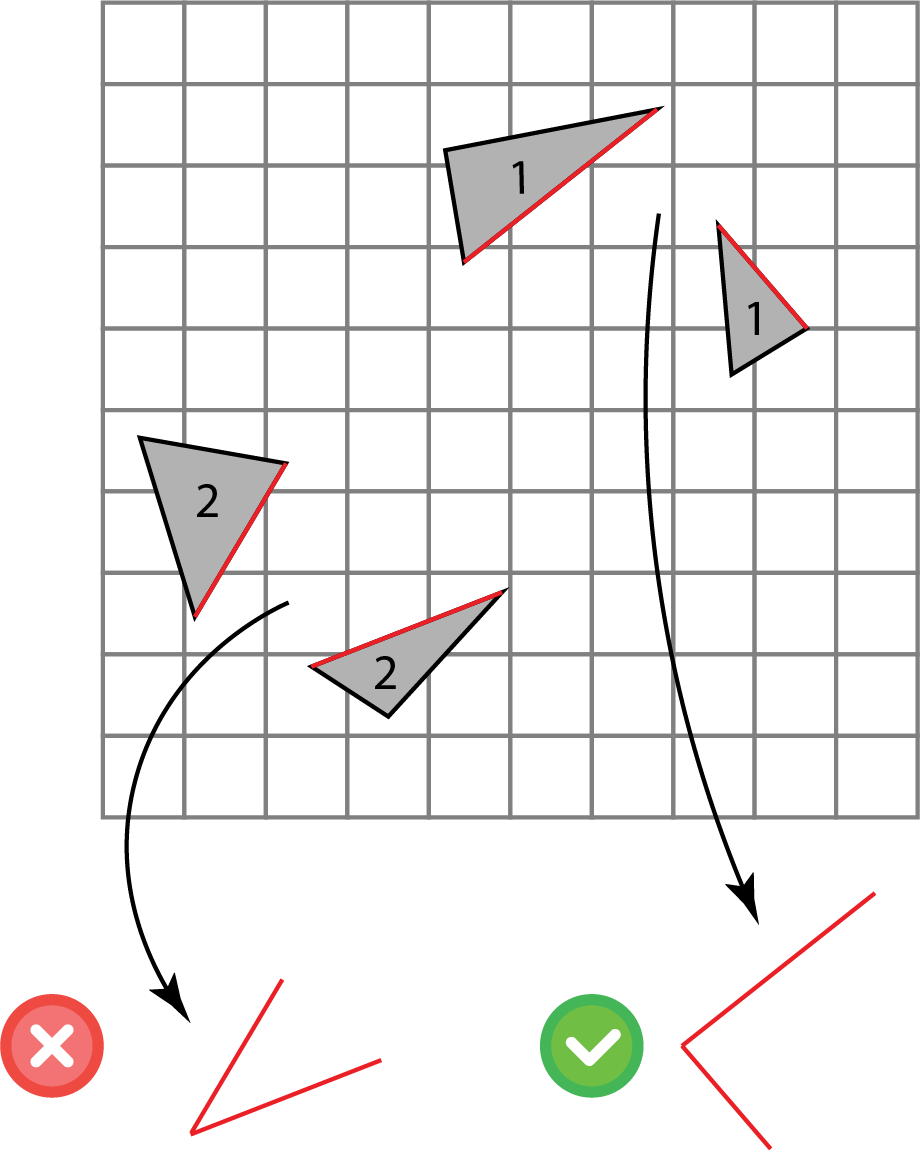
\includegraphics[width=9cm]{figures/seamless/angle.png}
\caption[The Angle Requirement]{The transition function $g_{ij}$, described by equation \ref{transition_g_ij}, should impose a $\frac{\pi}{2}k$ rotation between the two half edges.}
\label{fig:angle_req}
\end{figure}
\begin{figure}[ht]
\centering
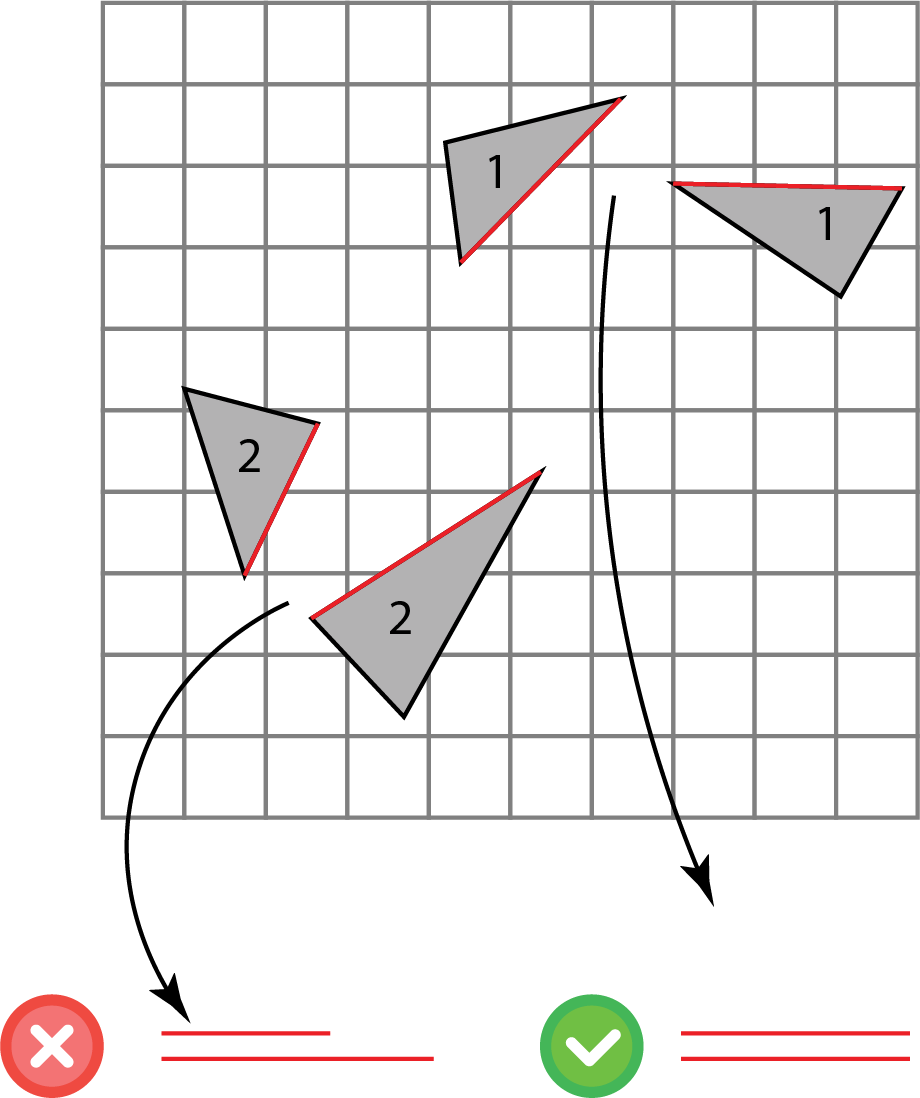
\includegraphics[width=9cm]{figures/seamless/length.png}
\caption[The Length Requirement]{The transition function $g_{ij}$, described by equation \ref{transition_g_ij}, should implicitly match the length of the two half edges.}
\label{fig:length_req}
\end{figure}
\subsection{Singular Points Condition}
\label{label:singular_points_cond}
Before we define what the singular-points condition is, we first have to define how a singular vertex is characterized on the parametrization domain. A singular-vertex (valence $\neq 4$) on the mesh's surface, will be characterized on the parametrization domain by a non-zero angular defect. The angular defect is measured by $2\pi - \sum_{i=1}^k \theta_i$ and $\pi - \sum_{i=1}^k \theta_i$ for interior and boundary surface vertices, respectively, where $k$ is the number of twin-vertices on the the parametrization domain that correspond to the singular-vertex on the mesh's surface, and $\theta_i$ is the angle adjacent to twin-vertex $v_i$.
Having the right definitions, the singular-points condition is require that all twin-vertices of singular points will be located on integer locations. Formally, given the set $V_i$ of all twin-vertices on the domain the that correspond to the same singular vertex $v_i$ on the mesh's surface, we require that:
\begin{equation}\label{eq:singular_points_cond}
\begin{split}
\forall u \in V_i: u \in \mathbb{Z}^2
\end{split}
\end{equation}
Figure \ref{fig:singular_points_req} demonstrate this condition visually.
\begin{figure}[ht]
\centering
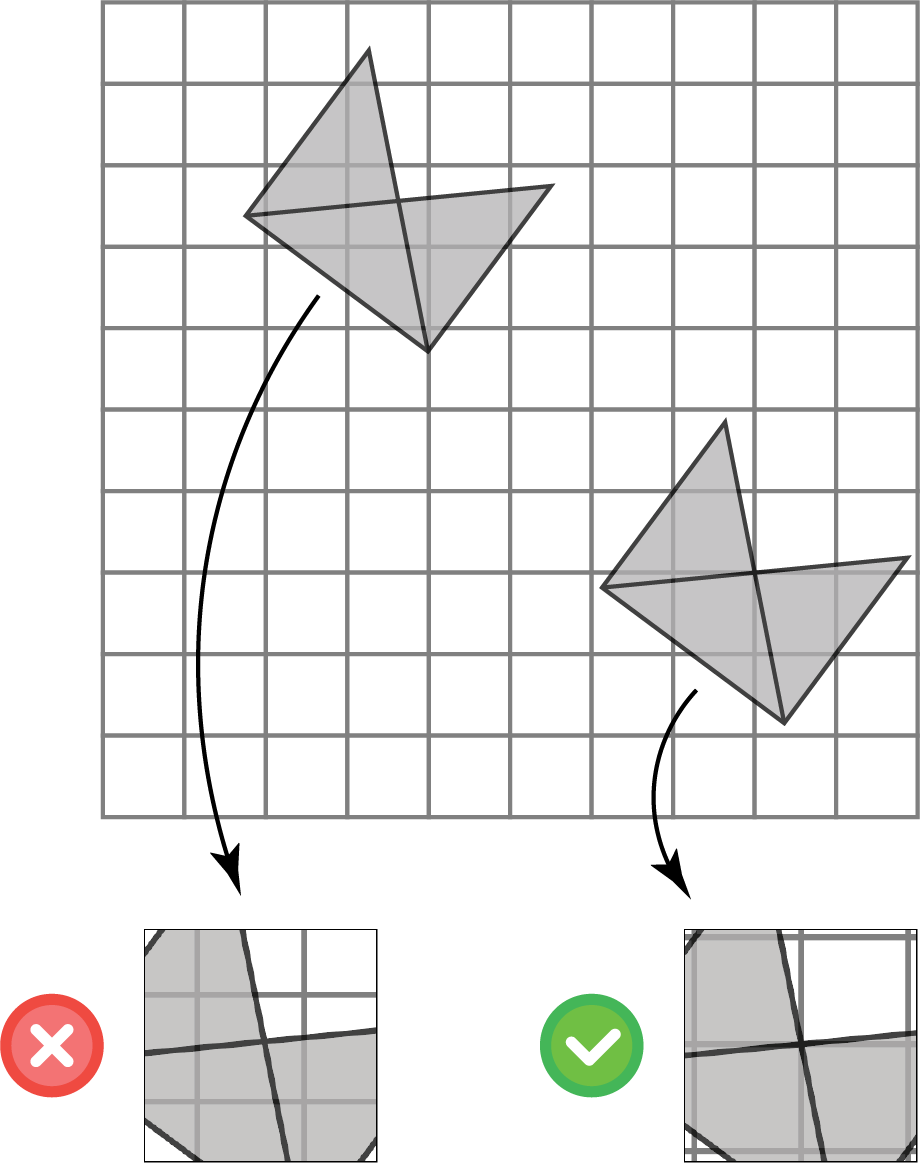
\includegraphics[width=9cm]{figures/singular_points/singularity.png}
\caption[The Singular Points Requirement]{Domain vertices that correspond to the same singular point should be positioned at a integer locations (grid points). In this illustration, the angular defect is $\frac{\pi}{2}$.}
\label{fig:singular_points_req}
\end{figure}
\subsection{Consistent Orientation Condition}
\label{label:consistent_otrientation_cond}
All triangles on the parameterization domain should have the same orientation. In other words, the transition function should not allow triangle flips. Figure \ref{fig:orientation_req} demonstrate this condition visually.
\begin{figure}[ht]
\centering
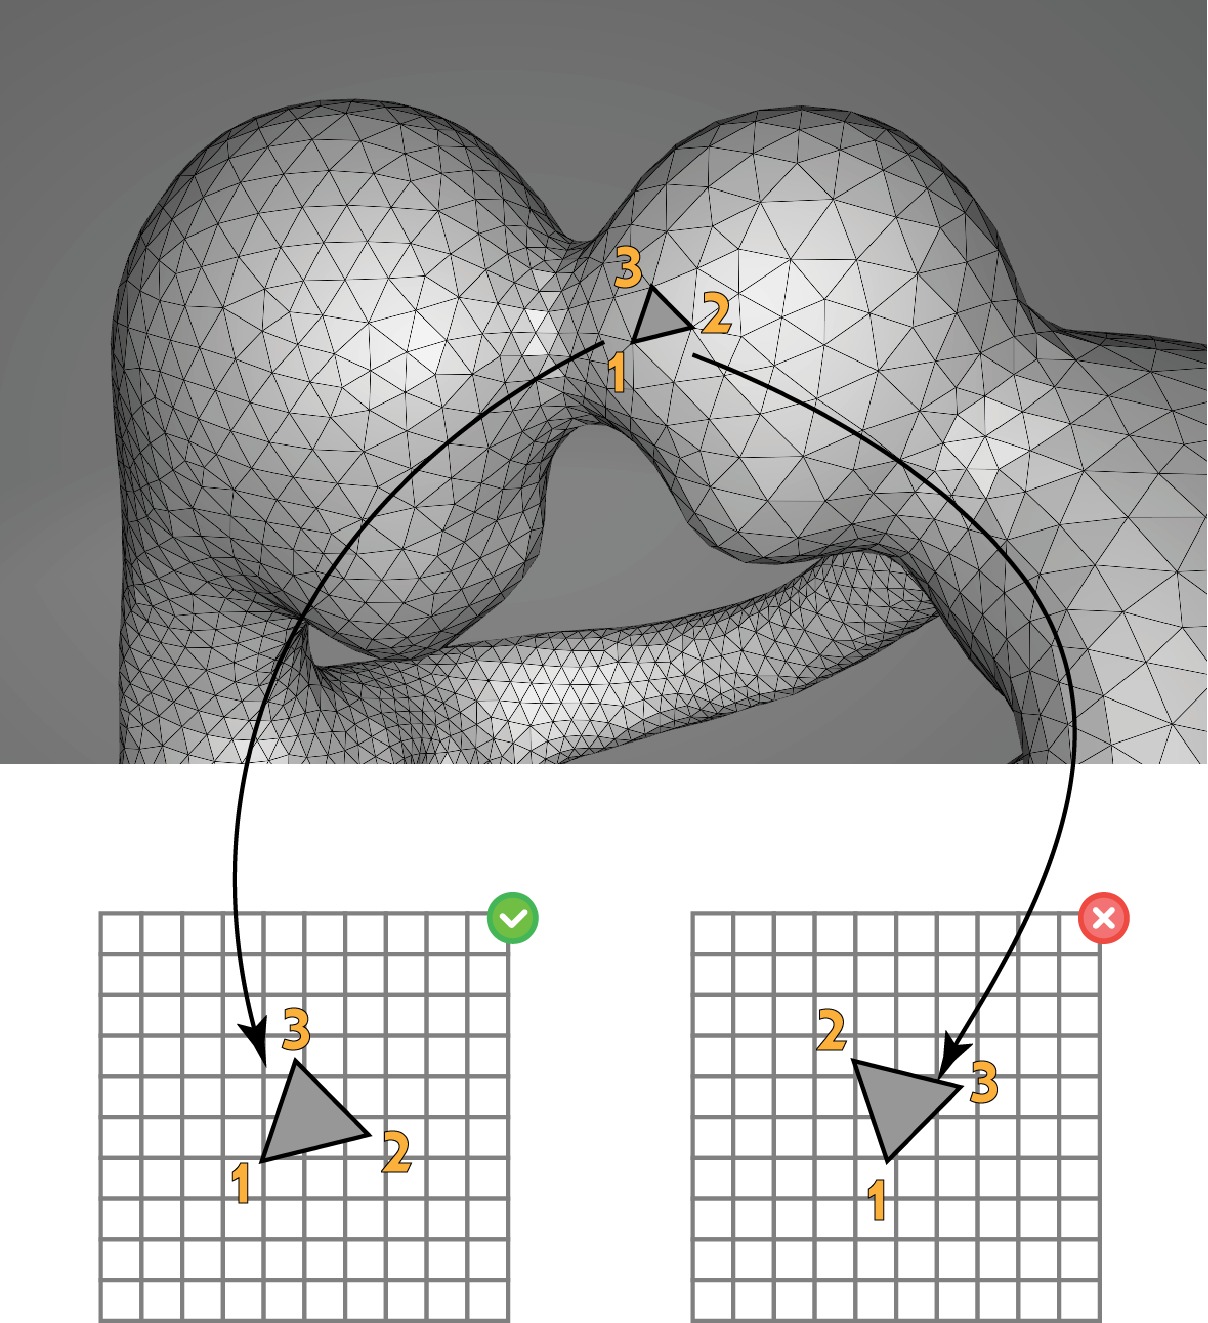
\includegraphics[width=9cm]{figures/orientation/orientation.png}
\caption[The Orientation Requirement]{The left triangle follows the same counter clockwise orientation as its image on the mesh's surface. On the other hand, the vertices of the triangle on the right follows a clockwise orientation.}
\label{fig:orientation_req}
\end{figure}
\section{Quad Distortion}
\label{label:quad_distortion_cond}
The fulfilment of the integer-grid maps conditions do guarantee that the isolines of the 2D Cartesian grid forms a valid quad-mesh on the 3D mesh's surface, however, we do have to consider at what cost. There are many possible integer-grid maps that transform a given triangle-mesh into a quad-mesh. Amongst them, we would like to pick the one that satisfies our desired set of additional requirements. In order to meet this desiderata, we have to pay with shape distortion of the triangles that make up the parametrization domain. Ultimately, we would like to find a map that fits our needs and minimizes the triangles distortion, since a distorted triangle renders a distorted isoline on the input mesh surface, which eventually affects the quality of the extracted quads that correspond to that triangle. Therefore, in addition to the integer-grid maps conditions, we add an additional implicit core requirement, which demands to find a mapping that minimizes triangle distortion. Figure \ref{fig:distortion_req} demonstrate this requirement visually.
\begin{figure}[ht]
\centering
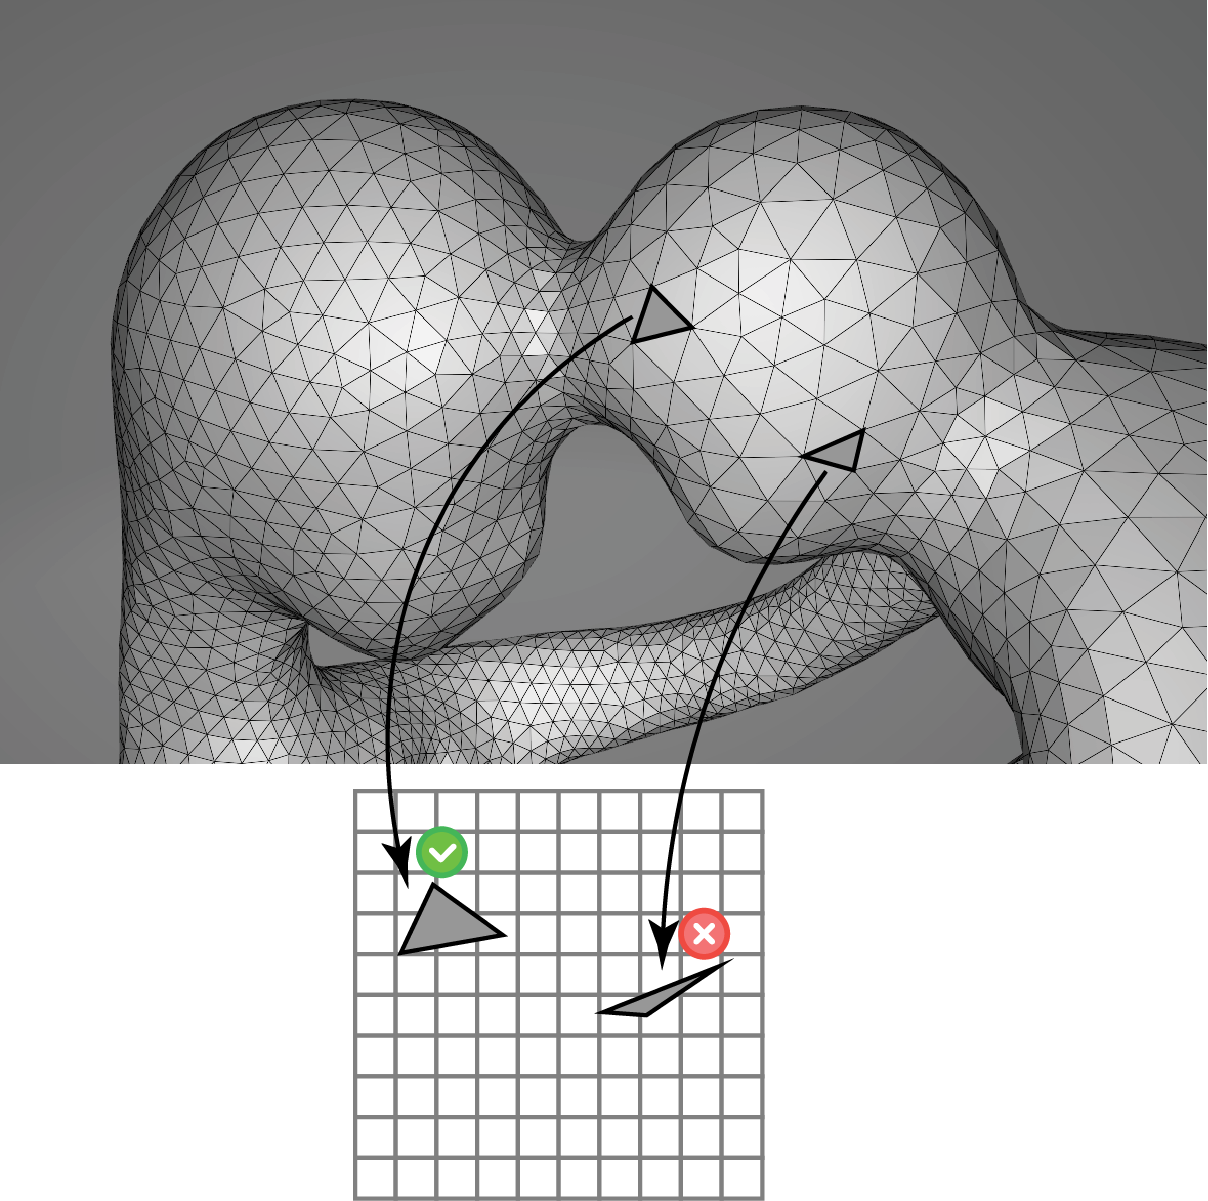
\includegraphics[width=9cm]{figures/distortion/distortion.png}
\caption[The Orientation Requirement]{The left triangle has a little shape distortion compared with its original version on the input-mesh's surface, in contrast with the right triangle, which clearly express a high shape distortion compared with its original version}
\label{fig:distortion_req}
\end{figure}
\section{Smooth Objective Functions}
In this section, we present our smooth objective function formulations for Conditions \ref{label:seamless_cond}, \ref{label:singular_points_cond}, \ref{label:consistent_otrientation_cond} and requirement \ref{label:quad_distortion_cond} presented in the previous sections.
\subsection{The Seamless Condition's Objective Functions}
The seamless condition can be expressed by three smooth objective (penalty) functions $P_{angle}$, $P_{length}$ and $P_{translation}$, that penalize violations in angle, length and translation, respectively, for a given pair of half-edges.
\paragraph{Angle Penalty}
Given two half-edges $e^i = \left(v^i_1,v^i_2\right)$ and $e^j = \left(v^j_1,v^j_2\right)$ in the parametrization domain, we define $P_{angle}$ as follows:
\begin{equation}\label{angle_penalty}
\begin{split}
P_{angle}\left(e^i,e^j\right) = \mathrm{sin} \bigg( 4\Big(\theta\left(e^i\right) - \theta\left(e^j\right)\Big) - \frac{\pi}{2}\bigg) + 1
\end{split}
\end{equation}
Where given that $k\in\left\{i,j\right\}$, $v^k_1$ and $v^k_2$ represent the first and second vertices, respectively, that constitutes half-edge, $\theta\left(e^k\right) = \mathrm{atan2}\Big(y\left(v^k_2\right) - y\left(v^k_1\right), x\left(v^k_2\right) - x\left(v^k_1\right)\Big)$ is the angle formed by half-edge $k$ with the positive \emph{x-axis} direction, and $x\left(v\right)$, $y\left(v\right)$ return the $x$ and $y$ coordinates, respectively, of an input vertex $v$. Please note that $\theta\left(e^i\right) - \theta\left(e^j\right)$ yields the signed angle between the two half-edges. Figure \ref{fig:angle_penalty} shows a plot of the angle penalty function for a range of $\theta$ values. It is easy to see that the angle penalty is minimized when the angle discrepancy between the two half-edges if an integer multiple of $\frac{\pi}{2}$, as required by the seamless condition.
\begin{figure}[ht]
\centering
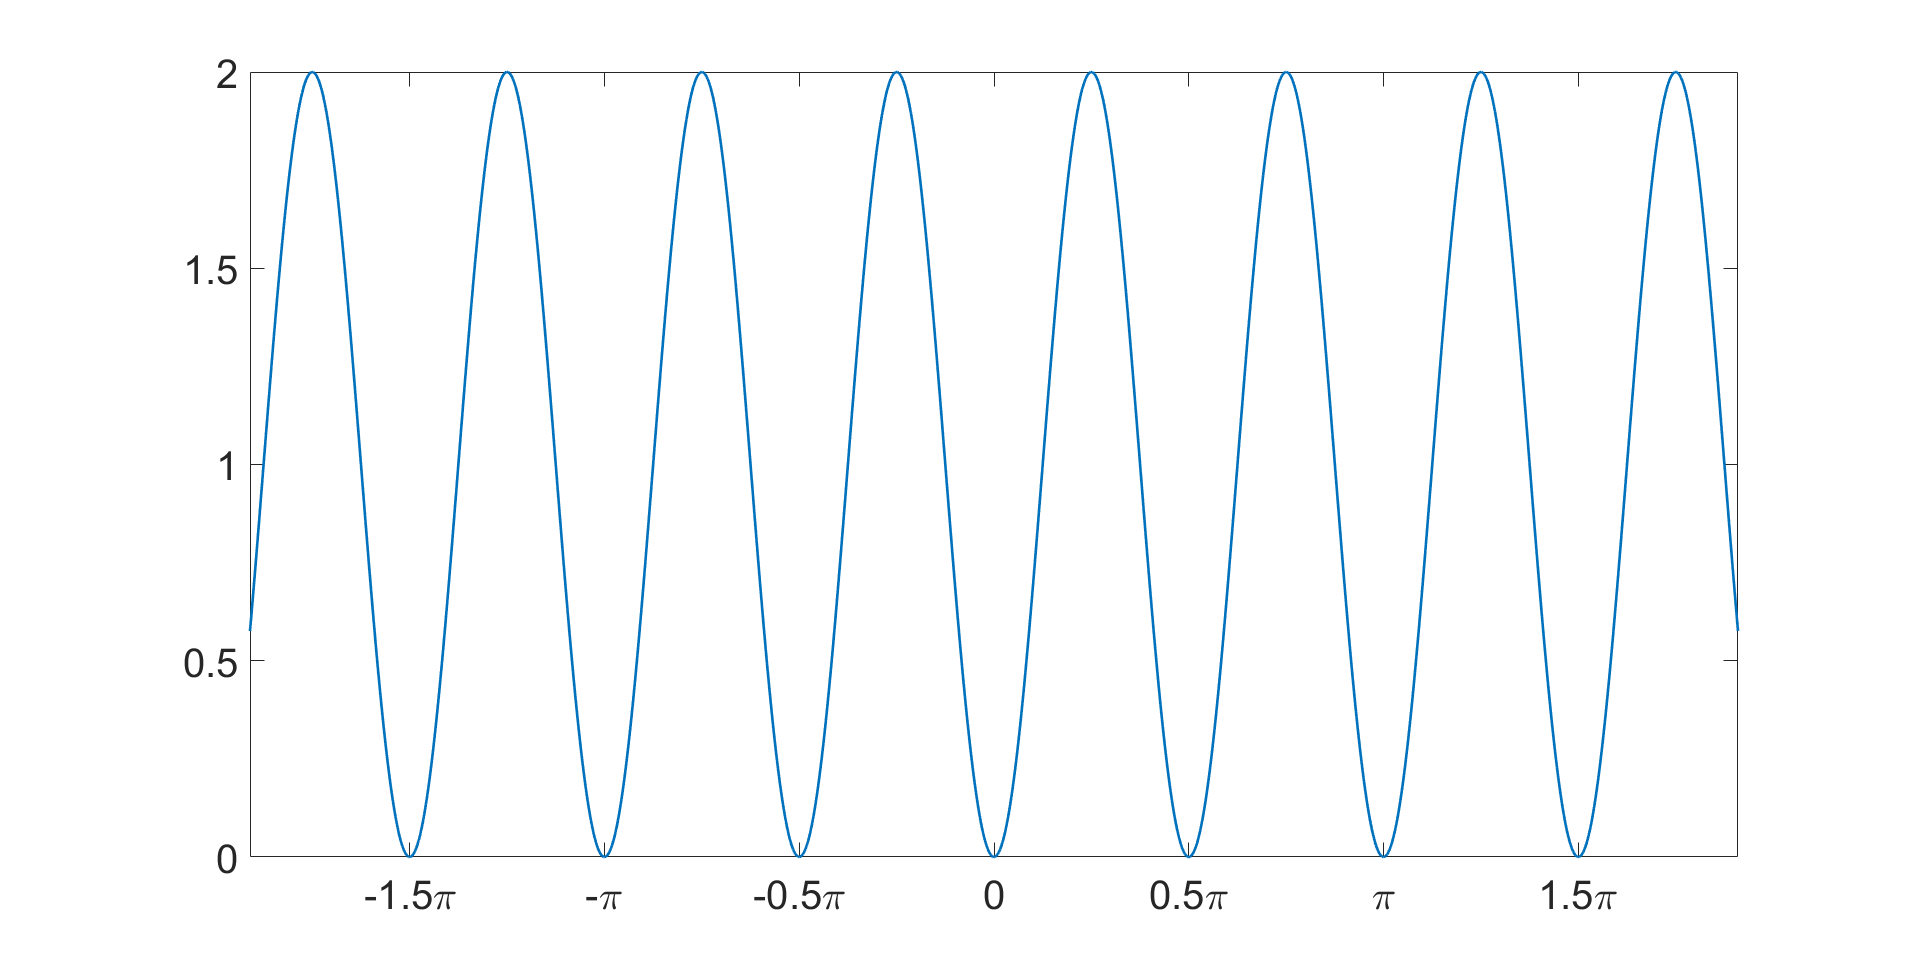
\includegraphics[width=15cm]{figures/seamless/angle_penalty.png}
\caption[Angle Penalty Function]{A plot of the angle penalty function. The penalty is zero for half-edges with angle discrepancy of integer multiples of $\frac{\pi}{2}$}
\label{fig:angle_penalty}
\end{figure}
\paragraph{Length Penalty}
Given two half-edges $e^i = \left(v^i_1,v^i_2\right)$ and $e^j = \left(v^j_1,v^j_2\right)$ in the parametrization domain, we define $P_{length}$ as follows:
\begin{equation}\label{length_penalty}
\begin{split}
P_{length}\left(e^i,e^j\right) = \left(\norm{e^i}_2^2 - \norm{e^j}_2^2\right)^2
\end{split}
\end{equation}
The length penalty measures the discrepancy between the Euclidean length of the two half-edges. It is a convex function (its Hessian is positive semi-definite) with multiple global minimum points associated with function value of $0$. Therefore, It is easy to see that the length penalty is minimized when the length discrepancy between the two half-edges is absolutely zero, as required by the seamless condition.
\paragraph{Translation Penalty}
Given two half-edges $e^i = \left(p^i_1,p^i_2\right)$ and $e^j = \left(p^j_1,p^j_2\right)$ in the parametrization domain, we define $P_{translation}$ as follows:
\begin{equation}\label{eq:translation_penalty}
\begin{split}
P_{translation}\left(e^i,e^j\right) = \mathrm{sin} \Big( 2\pi\Delta_x\big(e^i,e^j\big) - \frac{\pi}{2}\Big) + \mathrm{sin} \Big( 2\pi\Delta_y\big(e^i,e^j\big) - \frac{\pi}{2}\Big) + 2
\end{split}
\end{equation}
Where $\Delta_x\big(e^i,e^j\big) = \mathrm{x}\left(v^i_1\right) - \mathrm{x}\left(v^j_1\right)$ and $\Delta_y\big(e^i,e^j\big) = \mathrm{y}\left(v^i_1\right) - \mathrm{y}\left(v^j_1\right)$ represent the Manhattan distance between the two twin-vertices $v^i_1$ and $v^j_1$. Since the two sine terms in equation \ref{eq:translation_penalty} achieve their minimum value only for integer $\Delta_x$ and $\Delta_y$, it means that it penalize non-integer distances. Therefore, it is easy to see that the translation penalty is minimized when the two twin-vertices are integer distance apart, as required by the seamless condition. Figure \ref{fig:translation_penalty} shows a plot of the translation penalty function for a 2D domain patch of $\Delta_x$ and $\Delta_y$ values. 
\begin{figure}[ht]
\centering
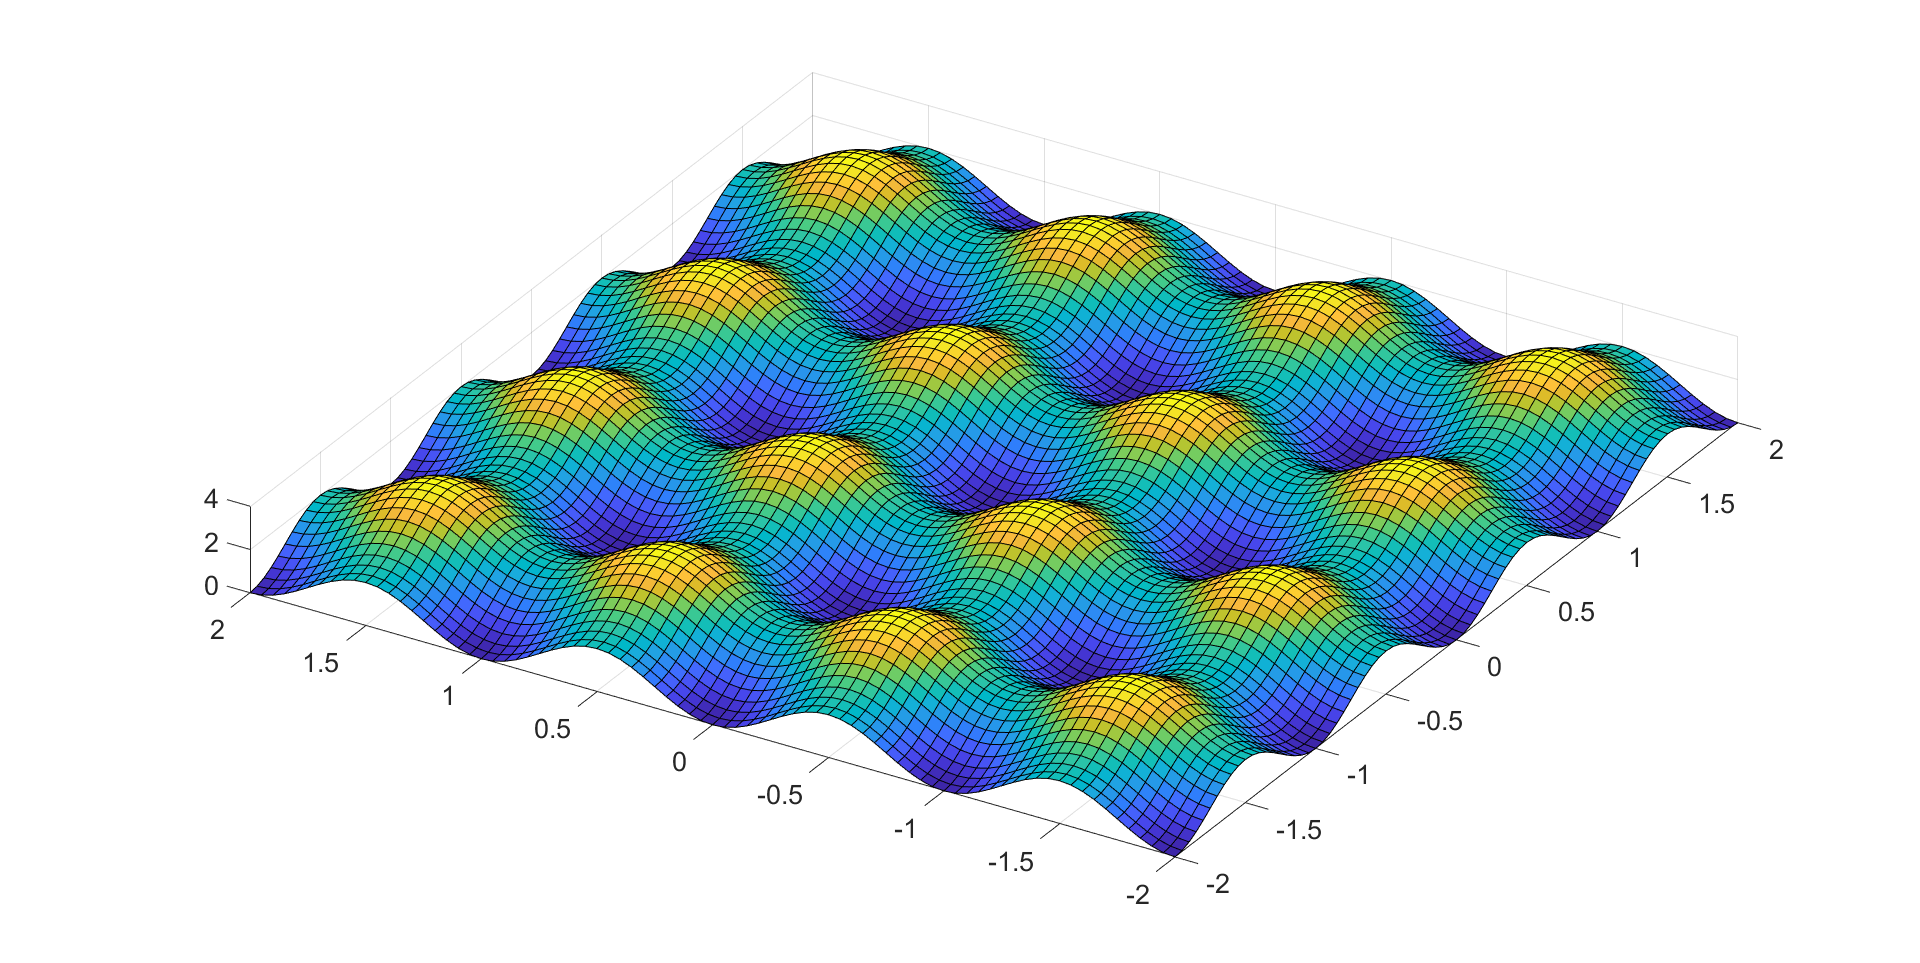
\includegraphics[width=15cm]{figures/seamless/translation_penalty.png}
\caption[Translation Penalty Function]{A plot of the translation penalty function for the domain range $\left(-2:2, -2:2\right)$. As can be seen, global minimum points are located at integer locations, which represent integer translation}
\label{fig:translation_penalty}
\end{figure}
\subsection{The Singular-Points Condition's Objective Functions}
The singular-points penalty function is applied on groups of twin-vertices on the parametrization domain, with non-zero angular defect (as defined in subsection \ref{label:singular_points_cond}). Given a group $V_i$ of twin-vertices that correspond to a singular points, the singular-points penalty function applied on that group is defined as follows:

\begin{equation}\label{eq:singular_points_penalty}
\begin{split}
P_{singular}\left(V_i\right) = \sum_{u \in V_i} \bigg( \mathrm{sin} \Big( 2\pi\mathrm{x}\big(u_i\big) - \frac{\pi}{2}\Big) + \mathrm{sin} \Big( 2\pi\mathrm{y}\big(u_i\big) - \frac{\pi}{2}\Big) + 2 \bigg)
\end{split}
\end{equation}

\begin{figure}[ht]
\centering
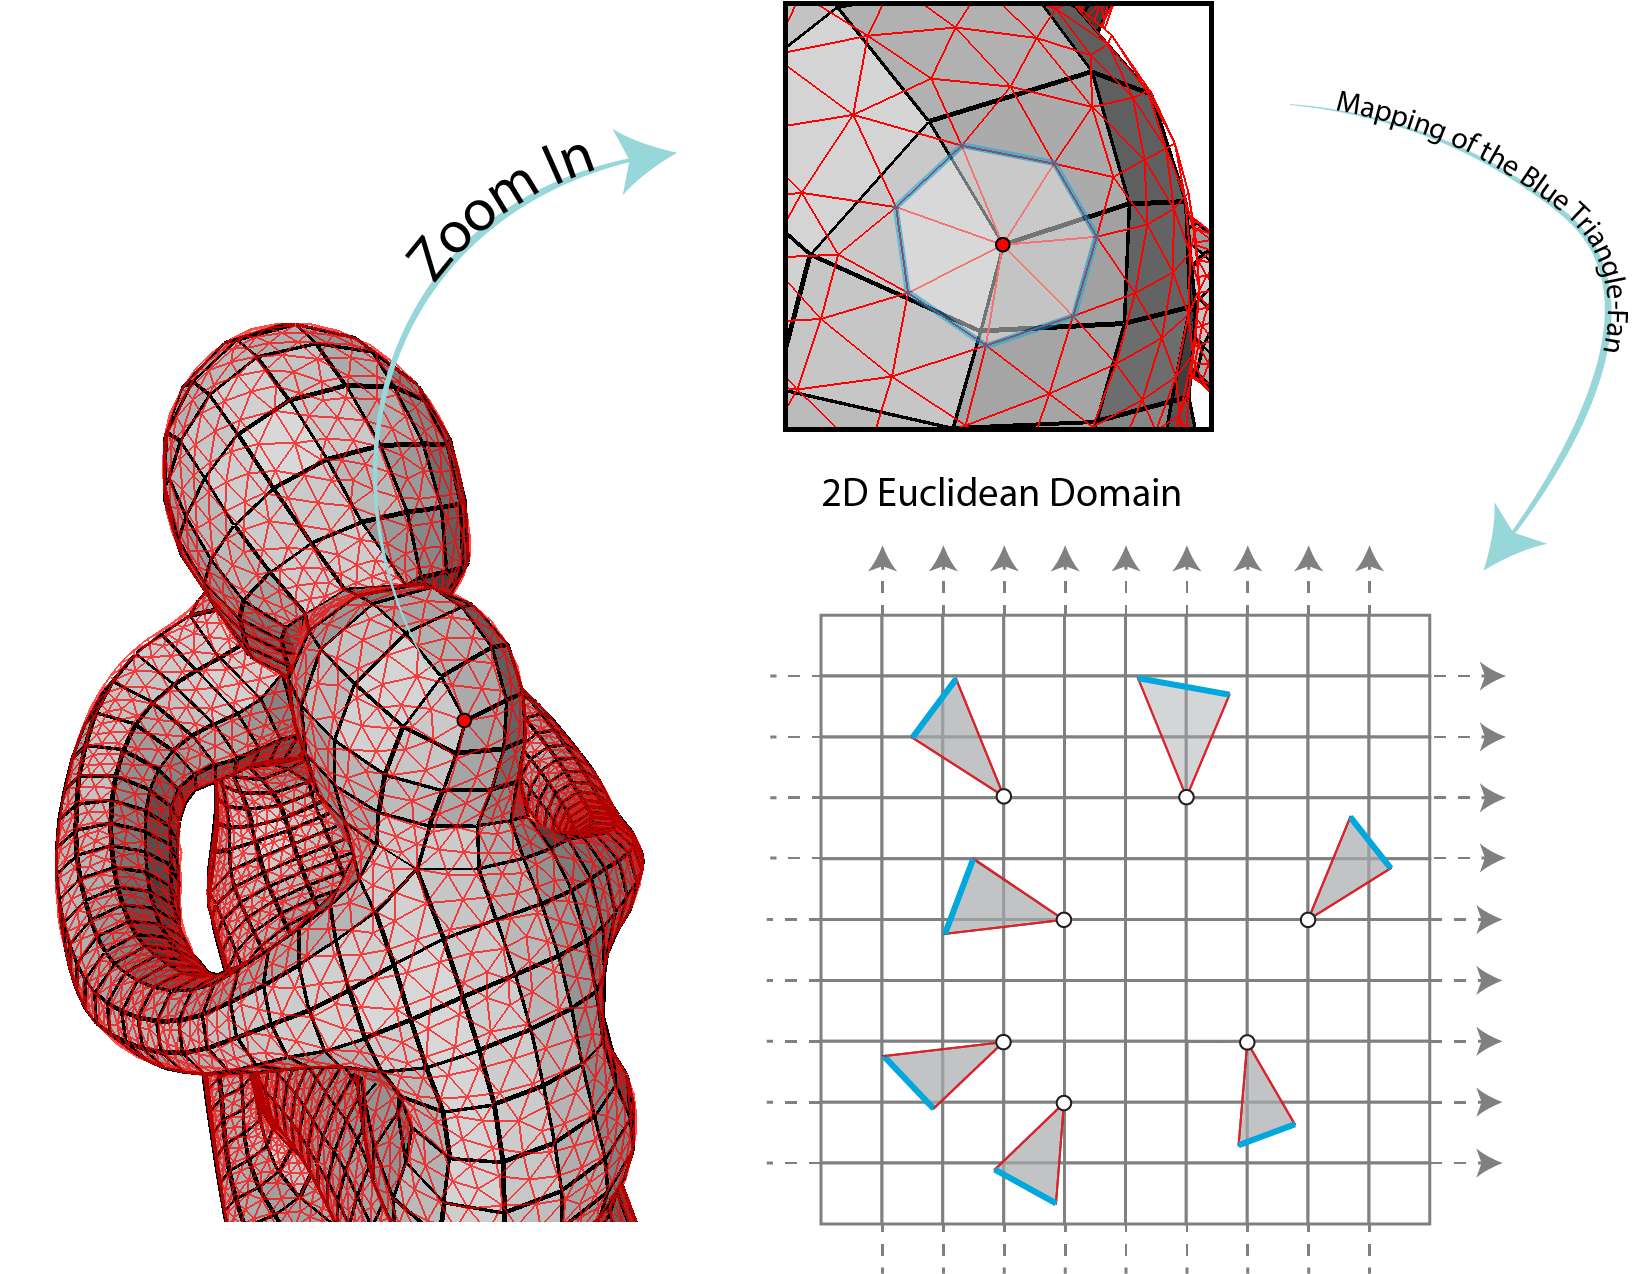
\includegraphics[width=16cm]{figures/singular_points/singular_points_penalty.png}
\caption[Translation Penalty Function]{A plot of the translation penalty function for the domain range $\left(-2:2, -2:2\right)$. As can be seen, global minimum points are located at integer locations, which represent integer translation}
\label{fig:singular_points_penalty}
\end{figure}